\documentclass{article}
\usepackage[T1]{fontenc}
\usepackage{amsmath,amssymb}
\usepackage[paperwidth=195mm,paperheight=58mm,margin=0mm]{geometry}
\usepackage{tikz}
\usetikzlibrary{arrows.meta,backgrounds,calc,fit,positioning}

% Low-saturation, color-blind-safe palette for print and screen.
\definecolor{ink}{HTML}{243746}
\definecolor{muted}{HTML}{61717D}
\definecolor{linegray}{HTML}{788995}
\definecolor{panel}{HTML}{F7F9FA}
\definecolor{blue}{HTML}{2E668F}
\definecolor{bluefill}{HTML}{E7F0F7}
\definecolor{teal}{HTML}{287D75}
\definecolor{tealfill}{HTML}{E7F3F0}
\definecolor{amber}{HTML}{AD7416}
\definecolor{amberfill}{HTML}{FFF3D8}

\tikzset{
  external/.style={draw=linegray, fill=panel, rounded corners=1.4mm,
    line width=.55pt, align=center, inner xsep=1mm,
    font=\sffamily\scriptsize, text=ink},
  module/.style={draw=blue, fill=bluefill, rounded corners=1.4mm,
    line width=.75pt, align=center, inner xsep=1mm,
    font=\sffamily\scriptsize, text=ink},
  inverse/.style={draw=teal, fill=tealfill, rounded corners=1.4mm,
    line width=.75pt, align=center, inner xsep=1mm,
    font=\sffamily\scriptsize, text=ink},
  recovery/.style={draw=amber, fill=amberfill, rounded corners=1.4mm,
    line width=.75pt, align=center, inner xsep=1mm,
    font=\sffamily\scriptsize, text=ink},
  safetybox/.style={draw=amber, fill=amberfill, rounded corners=1.4mm,
    line width=.9pt, align=center, inner xsep=1mm,
    font=\sffamily\scriptsize, text=ink},
  flow/.style={-{Stealth[length=1.8mm,width=1.35mm]}, draw=linegray,
    line width=.65pt, rounded corners=1.2mm},
  info/.style={-{Stealth[length=1.8mm,width=1.35mm]}, draw=blue,
    line width=.72pt, rounded corners=1.2mm},
  command/.style={-{Stealth[length=1.8mm,width=1.35mm]}, draw=teal,
    line width=.72pt, rounded corners=1.2mm},
  shiftarrow/.style={-{Stealth[length=1.8mm,width=1.35mm]}, draw=amber,
    line width=.72pt, dashed, rounded corners=1.2mm},
  edgeLabel/.style={font=\sffamily\tiny, text=muted, fill=white,
    inner xsep=.8mm, inner ysep=.25mm},
  badge/.style={circle, minimum size=3.6mm, inner sep=0pt, draw=blue,
    fill=white, line width=.55pt, font=\sffamily\tiny\bfseries, text=blue}
}

\begin{document}
\pagestyle{empty}
\noindent
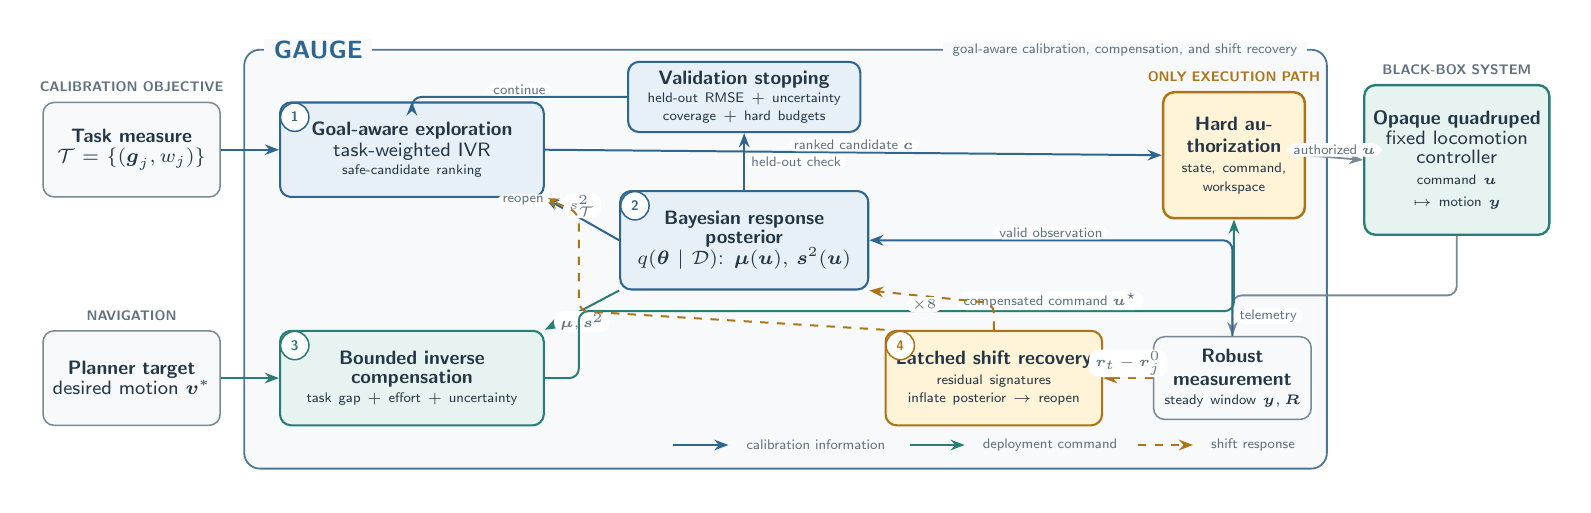
\begin{tikzpicture}[x=1mm,y=1mm]
  % Fix the artwork to the original 195 x 58 mm canvas.  The paper includes
  % this PDF by width, so preserving the aspect ratio preserves display height.
  \useasboundingbox (0,0) rectangle (195,58);

  % Method envelope: the opaque controller and robot remain explicitly external.
  \begin{scope}[on background layer]
    \fill[panel, rounded corners=2mm] (27.5,2.0) rectangle (165.0,55.2);
    \draw[blue!55!linegray, rounded corners=2mm, line width=.65pt]
      (27.5,2.0) rectangle (165.0,55.2);
  \end{scope}
  \node[anchor=west, fill=panel, inner xsep=1.2mm, inner ysep=.2mm,
        font=\sffamily\small\bfseries, text=blue] at (30.0,55.2) {GAUGE};
  \node[anchor=east, fill=panel, inner xsep=1.2mm, inner ysep=.2mm,
        font=\sffamily\tiny, text=muted] at (162.5,55.2)
        {goal-aware calibration, compensation, and shift recovery};

  % External task and planner inputs.
  \node[external, text width=20.5mm, minimum height=12mm] (task)
        at (13.2,42.5) {\textbf{Task measure}\\[-.3mm]
        $\mathcal{T}=\{(\boldsymbol g_j,w_j)\}$};
  \node[font=\sffamily\tiny\bfseries, text=muted, anchor=south]
        at (task.north) {CALIBRATION OBJECTIVE};

  \node[external, text width=20.5mm, minimum height=12mm] (goal)
        at (13.2,13.5) {\textbf{Planner target}\\[-.3mm]
        desired motion $\boldsymbol v^{*}$};
  \node[font=\sffamily\tiny\bfseries, text=muted, anchor=south]
        at (goal.north) {NAVIGATION};

  % Four scientific components of GAUGE.
  \node[module, text width=31.5mm, minimum height=12mm] (explore)
        at (48.8,42.5) {\textbf{Goal-aware exploration}\\[-.2mm]
        task-weighted IVR\\[-.5mm]{\tiny safe-candidate ranking}};
  \node[badge] at ([xshift=2mm,yshift=-2mm]explore.north west) {1};

  \node[module, text width=27.5mm, minimum height=7.5mm] (stop)
        at (91.0,49.2) {\textbf{Validation stopping}\\[-.5mm]
        {\tiny held-out RMSE $+$ uncertainty}\\[-.6mm]
        {\tiny coverage $+$ hard budgets}};

  \node[module, text width=29.5mm, minimum height=12.5mm] (posterior)
        at (91.0,31.0) {\textbf{Bayesian response}\\[-.4mm]\textbf{posterior}\\[-.2mm]
        $q(\boldsymbol\theta\mid\mathcal D)$: $\boldsymbol\mu(\boldsymbol u),\,\boldsymbol s^2(\boldsymbol u)$};
  \node[badge] at ([xshift=2mm,yshift=-2mm]posterior.north west) {2};

  \node[inverse, text width=31.5mm, minimum height=12mm] (compensate)
        at (48.8,13.5) {\textbf{Bounded inverse}\\[-.4mm]\textbf{compensation}\\[-.3mm]
        {\tiny task gap $+$ effort $+$ uncertainty}};
  \node[badge, draw=teal, text=teal] at
        ([xshift=2mm,yshift=-2mm]compensate.north west) {3};

  \node[recovery, text width=25.5mm, minimum height=12mm] (recover)
        at (122.7,13.5) {\textbf{Latched shift recovery}\\[-.3mm]
        {\tiny residual signatures}\\[-.5mm]
        {\tiny inflate posterior $\rightarrow$ reopen}};
  \node[badge, draw=amber, text=amber] at
        ([xshift=2mm,yshift=-2mm]recover.north west) {4};

  % A single authorization path separates statistical ranking from execution.
  \node[safetybox, text width=16mm, minimum height=16mm] (safety)
        at (153.2,41.8) {\textbf{Hard authorization}\\[-.2mm]
        {\tiny state, command,}\\[-.5mm]{\tiny workspace}};
  \node[font=\sffamily\tiny\bfseries, text=amber, anchor=south]
        at (safety.north) {ONLY EXECUTION PATH};

  \node[external, draw=teal, fill=tealfill, line width=.85pt,
        text width=21.5mm, minimum height=19mm] (robot)
        at (181.5,41.2) {\textbf{Opaque quadruped}\\[-.2mm]
        fixed locomotion\\[-.4mm]controller\\[-.2mm]
        {\tiny command $\boldsymbol u$ $\mapsto$ motion $\boldsymbol y$}};
  \node[font=\sffamily\tiny\bfseries, text=muted, anchor=south]
        at (robot.north) {BLACK-BOX SYSTEM};

  \node[external, text width=18mm, minimum height=10.5mm] (measure)
        at (153.0,13.5) {\textbf{Robust measurement}\\[-.4mm]
        {\tiny steady window $\boldsymbol y,\boldsymbol R$}};

  % Active calibration and posterior update.
  \draw[info] (task.east) -- (explore.west);
  \draw[info] (explore.east) -- node[edgeLabel, above] {ranked candidate $\boldsymbol c$}
        (safety.west);
  \draw[flow] (safety.east) -- node[edgeLabel, above] {authorized $\boldsymbol u$}
        (robot.west);
  \draw[flow] (robot.south) -- (181.5,24.0) -|
        node[edgeLabel, near end, right] {telemetry} (measure.north);
  \draw[info] (measure.north) |- node[edgeLabel, near end, above] {valid observation}
        (posterior.east);
  \draw[info] (posterior.north) -- node[edgeLabel, right] {held-out check} (stop.south);
  \draw[info] (stop.west) -| node[edgeLabel, near start, above] {continue}
        (explore.north);
  \draw[info] (posterior.west) -- node[edgeLabel, above] {$s^2_{\mathcal T}$}
        (explore.south east);

  % Deployment compensation uses the same posterior and the same hard gate.
  \draw[command] (goal.east) -- (compensate.west);
  \draw[command] (posterior.south west) -- node[edgeLabel, below]
        {$\boldsymbol\mu,\boldsymbol s^2$} (compensate.north east);
  \draw[command] (compensate.east) -- (70,13.5) -- (70,22.0) --
        node[edgeLabel, above, pos=.72] {compensated command $\boldsymbol u^{\star}$}
        (153.2,22.0) -- (safety.south);

  % Shift evidence is paired by monitor command; recovery is bounded and latched.
  \draw[shiftarrow] (measure.west) -- node[edgeLabel, above] {$\boldsymbol r_t-\boldsymbol r^0_j$}
        (recover.east);
  \draw[shiftarrow] (recover.north) -- (122.7,23.0) --
        node[edgeLabel, below, pos=.56] {$\times 8$}
        (posterior.south east);
  \draw[shiftarrow] (recover.north west) -- (70.0,22.0) -- (70.0,34.5) --
        node[edgeLabel, left, pos=.82] {reopen}
        (explore.south east);

  % Compact semantic key, intentionally inside the fixed canvas.
  \draw[info] (82.0,5.0) -- +(7.0,0)
        node[font=\sffamily\tiny, text=muted, right=1mm] {calibration information};
  \draw[command] (112.0,5.0) -- +(7.0,0)
        node[font=\sffamily\tiny, text=muted, right=1mm] {deployment command};
  \draw[shiftarrow] (141.0,5.0) -- +(7.0,0)
        node[font=\sffamily\tiny, text=muted, right=1mm] {shift response};
\end{tikzpicture}
\end{document}
